\subsection{Initial Setup \& Basic Exploration}\label{subsec:steps-1-3:-initial-setup-&-basic-exploration}
Since a Linux environment is needed to explore the \texttt{/proc} filesystem
and for POSIX compliance, the first step was to install a Virtual Machine (VM)
and a Linux ISO to run on it.
I already had an installation of Debian set up on my PC, so I used this as my testing environment.\\
I then used basic CLI tools to explore the \texttt{/proc} filesystem.
\begin{figure}[H]
    \centering
    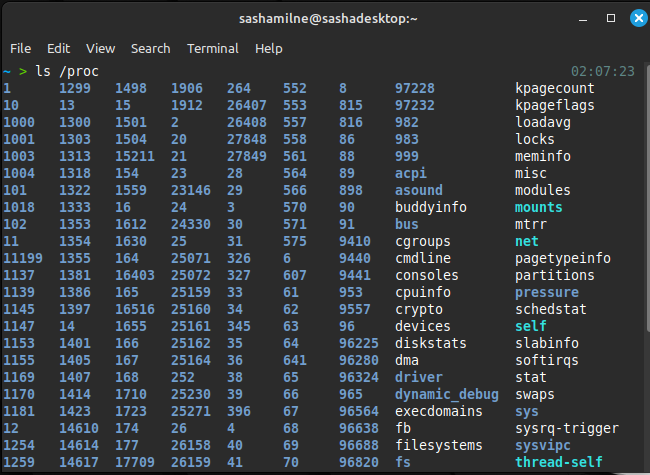
\includegraphics[width=0.7\textwidth]{../../screenshots/step1-lsproc}
    \caption{Exploring \texttt{/proc} using \texttt{ls}}
    \label{fig:step1-lsproc}
\end{figure}
\begin{figure}[H]
    \centering
    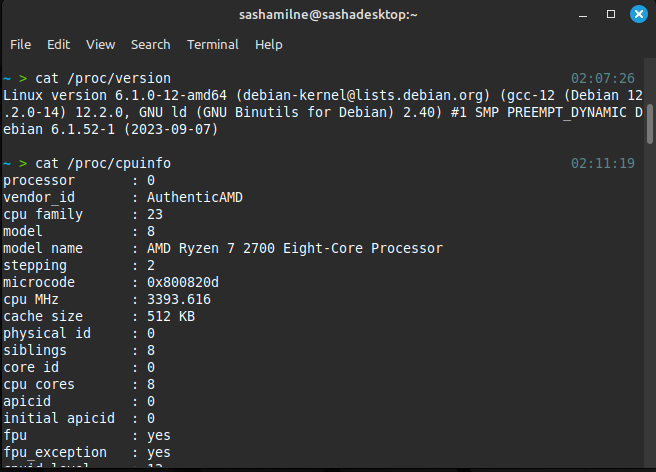
\includegraphics[width=0.7\textwidth]{../../screenshots/step2-3-catproc}
    \caption{Further exploration of \texttt{/proc} using \texttt{cat}}
    \label{fig:step2-3-catproc}
\end{figure}
\afterfloat
In \textit{Figure 1}, the CLI output of \texttt{ls /proc} can be observed.
This command lists all the contents of the \texttt{/proc} directory to \texttt{stdout}.
Each folder with a number contains information about a process referenced by its Process ID (PID)\@.
There are other miscellaneous files which contain critical system info which can be observed.\\
In \textit{Figure 2}, two such files are examined, \texttt{version} and \texttt{cpuinfo}, using \texttt{cat}.
Here, information is displayed onto the CLI about what version of \texttt{proc} is being used
and information about the CPU\@.
For example, I allocated 8 of my 16 threads in my Ryzen 7 2700,
and we can observe the system seeing 8 CPU cores available.

\subsection{Finding Process Info}\label{subsec:finding-process-info}
The goal of the next activity was to find the PID of the shell and explore its process status.
We used \texttt{bash} as the shell and \texttt{ps} to get the PID\@.
\begin{figure}[H]
    \centering
    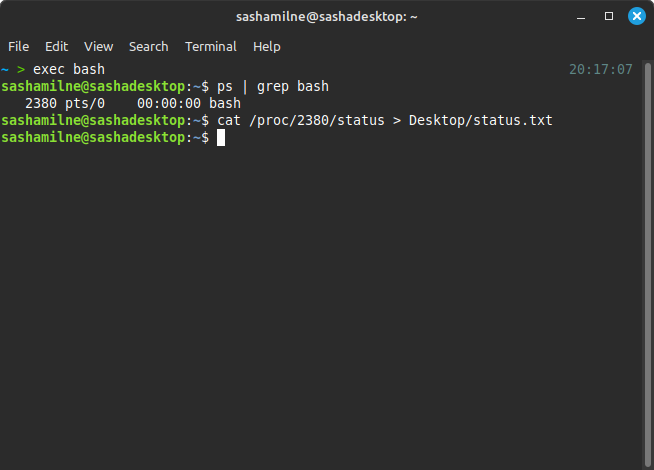
\includegraphics[width=0.7\textwidth]{../../screenshots/step4-ps}
    \caption{Finding the PID of the shell and getting its status}
    \label{fig:step4-ps}
\end{figure}
\begin{figure}[H]
        \centering
        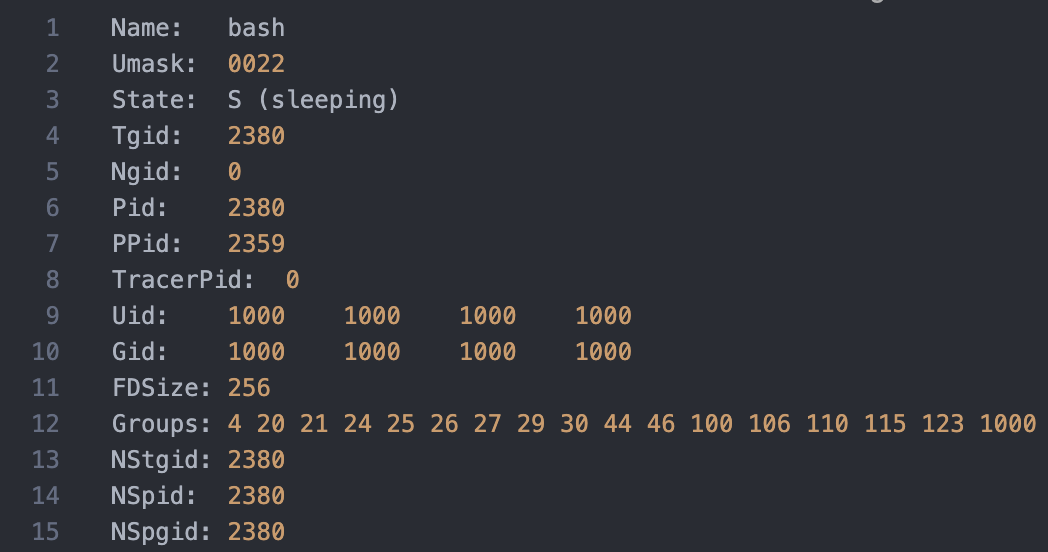
\includegraphics[width=0.7\textwidth]{../../screenshots/step5-status}
        \caption{Viewing the output file}
        \label{fig:step5-status}
    \end{figure}
\afterfloat
In \textit{Figure 3}, the shell PID is obtained using \texttt{ps}.
We then output the contents of \texttt{/proc/PID/status}, redirecting it into status.txt.
The full contents of this file can be found in \texttt{logs/status.log},
however, a screenshot is provided in \textit{Figure 4}.
From this figure, we can see that the process was sleeping at the
time of execution of \texttt{cat} along with many other details.

\subsection{Preparing Experiments \& Understanding Tools}\label{subsec:preparing-experiments-&-understanding-tools}
The goal of this section is to explore the state changes of processes using specially created programs.
Using the provided \texttt{lab1.tar}, we will launch and observe other, more interesting programs.
\begin{figure}[H]
    \centering
    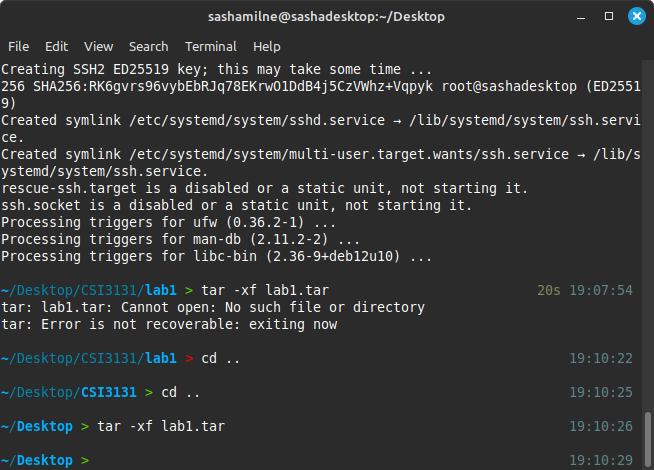
\includegraphics[width=0.7\textwidth]{../../screenshots/step6-tar}
    \caption{Extracting lab1 tar file}
    \label{fig:step6-extract-tar}
\end{figure}

\afterfloat
After extracting the contents of \texttt{lab1.tar},
I moved everything to my workspace directory and reorganized the
project structure for neatness.
Inside the \texttt{lab1} directory, there are three compiled binaries:
\texttt{procmon}, \texttt{calcloop}, and \texttt{cploop}.\\

\noindent
The purpose of the \texttt{procmon} program is to monitor the
status of a process given its PID\@.
The program accepts an argument \texttt{PID} which it then monitors
using the \texttt{proc} filesystem.\\

\noindent